Our intention is always to deliver maximum energy to the load, we, therefore, want the reflection coefficient in equation~\eqref{eqn:reflectioncoefficientatload} to be as small as possible. So we shall find the condition to deliver maximum power to the load i.e no reflection on the transmission line.

\section{Matched Condition of the Transmission Line}\label{lec:lec4}
Equation~\eqref{eqn:reflectioncoefficientatload} can be further expressed as
\begin{align*}
\Gamma_L = \frac{Z_L - Z_0}{Z_L + Z_0} = \frac{V^-}{V^+}
\end{align*}

It can be observed that when $Z_L = Z_0$, then there is no reflection from the load and hence maximum power is delivered to the generator. That is
\begin{align*}
\Gamma_L = \frac{V^-}{V^+} = 0\ (\text{when }Z_L = Z_0.) 
\end{align*}
Although $Z_0$ cannot be located on the transmission line, it does govern power flow in the transmission line. This condition that $Z_L = Z_0$ is called the \emph{matched condition}\index{matched condition} of the transmission line. The terminating impedance of the line is matched to the characteristic impedance. This condition is similar to the maximum power transfer theorem in a lumped circuit\textemdash\;where if the load impedance is equal to the conjugate of the generator impedance, maximum power is transferred from the generator to the load.
\begin{align*}
Z_L = Z_0 \quad (\text{Matched Load Condition})
\end{align*}
As the wave moves along the line, it sees $Z_0$. At $Z_L$, it suddenly sees an impedance discontinuity from $Z_0$ to $Z_L$ which is like a steep change because of that part of the energy that tends to get reflected by the generator on the transmission line. So, for maximum power transfer, the terminating load impedance must be equal to the characteristics impedance otherwise, maximum power transfer will not take place and there will always be reflection.

The reflection coefficient at any point on the transmission line from equation~\eqref{eqn:rfc} is given as:
\begin{align*}
\Gamma{(l)} = \frac{V^-e^{-\gamma l}}{V^+e^{\gamma l}} = \frac{\text{Backward wave}}{\text{Forward wave}}
\end{align*}
Therefore we can define the voltage and current equations at any point on the transmission line with respect to reflection coefficient $\Gamma(l)$. That is
\begin{align}
V(l) = V^+e^{\gamma l} + V^-e^{-\gamma l}\label{eqn:voltagefromloadchp4}\\
I(l) =\frac{V^+}{Z_0} e^{\gamma l} - \frac{V^-}{Z_0}e^{-\gamma l}\label{eqn:currentfromloadchp4}
\end{align}
Dividing equation~\ref{eqn:voltagefromloadchp4} by $V^+e^{\gamma l}$
\begin{dmath*}
\frac{V(l)}{ V^+e^{\gamma l}} = 1 + \frac{ V^-e^{-\gamma l}}{ V^+e^{\gamma l}}\quad\text{But }\Gamma(l)\text{ = }\frac{ V^-e^{-\gamma l}}{ V^+e^{\gamma l}}
= 1 + \Gamma(l)
\end{dmath*}
Therefore the voltage equation becomes
\begin{align}
V(l) = V^+e^{\gamma l} (1 + \Gamma(l))
\label{eqn:voltagelec4}
\end{align}
This gives the voltage at any point on the line. Similary, dividing equation~\ref{eqn:currentfromloadchp4} by $\frac{V^+}{Z_0} e^{\gamma l}$
\begin{dmath*}
\frac{I}{\frac{V^+}{Z_0} e^{\gamma l}} = 1 - \frac{\frac{V^-}{Z_0} e^{-\gamma l}}{\frac{V^+}{Z_0} e^{\gamma l}}
= 1 - \frac{V^-e^{-\gamma l}}{V^+e^{\gamma l}}
= 1 - \Gamma(l)
\end{dmath*}
Thus the current equation becomes
\begin{align}
I(l) = \frac{V^+}{Z_0} e^{\gamma l} (1 - \Gamma(l))
\label{eqn:currentlec4}
\end{align}
From lumped circuit analysis, we recall that $Z(l) = \frac{V(l)}{I(l)}$, thus, substituting equations~\eqref{eqn:voltagelec4} and~\eqref{eqn:currentlec4} we have
\begin{align*}
Z(l) &= \frac{V(l)}{I(l)}\\
&= \frac{V^+e^{\gamma l} (1 + \Gamma(l))}{ \dfrac{V^+}{Z_0} e^{\gamma l} (1 - \Gamma(l))}
\end{align*}
$V^+ e^{\gamma l}$ cancels out to give,
\begin{align}
Z(l) = Z_0\left[\frac{1 + \Gamma(l)}{1 - \Gamma(l)}\right]
\end{align}
$Z(l)$ \emph{is the impedance measured at any location of the transmission line. It is related to the reflection coefficient at any point and the characteristic impedance}. $\Gamma(l)$ is the reflection coefficient at any point on the transmission line. Hence $Z(l)$ and $\Gamma(l)$ have a one-to-one relationship at any point along the transmission line.

\section{Impedance Transformation Relationship}
Recall,
\begin{dmath*}
Z(l) = \frac{V(l)}{I(l)}\quad\text{Substituting equations~\eqref{eqn:voltagefromloadchp4} and~\eqref{eqn:currentfromloadchp4}}
= \frac{V^+e^{\gamma l} + V^-e^{-\gamma l}}{\frac{V^+}{Z_0}e^{\gamma l} - \frac{V^-}{Z_0}e^{-\gamma l}}
= Z_0\left[\frac{V^+e^{\gamma l} + V^-e^{-\gamma l}}{V^+e^{\gamma l} - V^-e^{-\gamma l}}\right]
\end{dmath*}
Dividing the numerator and denominator by $V^+e^{\gamma l}$ 
\begin{align*}
Z(l) = Z_0\left[\frac{1 + \frac{V^-e^{-\gamma l}}{V^+e^{\gamma l}}}{1 - \frac{V^-e^{-\gamma }}{V^+e^{\gamma }}}\right]
\end{align*}
Where $\Gamma_L = \frac{V^-}{V^+}$ and $\frac{e^{-\gamma l}}{e^{\gamma l}} = e^{-2\gamma l}$
\begin{align}
Z(l)= Z_0\left[\frac{1 + \Gamma_L e^{-2\gamma l}}{1 - \Gamma_L e^{-2\gamma l}}\right]
\end{align}
But $\Gamma_L
= \frac{Z_L - Z_0}{Z_L + Z_0}$,
\begin{align*}
Z(l) = Z_0 \left[\frac{1 + \left(\dfrac{Z_L - Z_0}{Z_L + Z_0}\right)e^{-2\gamma l}}{1 - \left(\dfrac{Z_L - Z_0}{Z_L + Z_0}\right)e^{-2\gamma l}}\right]
\end{align*}
Multiplying the numerator and denominator by $Z_L + Z_0 $ gives
\begin{dmath*}
Z(l) = Z_0 \left[\frac{(Z_L + Z_0) + (Z_L - Z_0)e^{-2\gamma l}}{(Z_L + Z_0) - (Z_L - Z_0)e^{-2\gamma l}}\right]
= Z_0 \frac{e^{-\gamma l}}{e^{-\gamma l}}\left[\frac{(Z_L + Z_0)e^{\gamma l} + (Z_L - Z_0)e^{-\gamma l}}{(Z_L + Z_0)e^{\gamma l} - (Z_L - Z_0)e^{-\gamma l}}\right]
= Z_0 \left[\frac{Z_L e^{\gamma l} + Z_0e^{\gamma l} + Z_L e^{-\gamma l} - Z_0e^{-\gamma l}}{Z_L e^{\gamma l} + Z_0e^{\gamma l} - Z_L e^{-\gamma l} + Z_0e^{-\gamma l}}\right]
\end{dmath*}
Collect like terms
\begin{align*}
Z(l) = Z_0 \left[\frac{Z_L(e^{\gamma l} + e^{-\gamma l}) + Z_0(e^{\gamma l} - e^{-\gamma l})}{Z_L (e^{\gamma l} - e^{-\gamma l}) + Z_0(e^{\gamma l} + e^{-\gamma l})}\right]
\end{align*}
Before we proceed let us recall that 
\begin{align*}
\cosh(\gamma l) = \frac{e^{\gamma l} + e^{-\gamma l}}{2}\\
2\cosh(\gamma l) = e^{\gamma l} + e^{-\gamma l}
\end{align*}
 and
\begin{align*}
\sinh(\gamma l) = \frac{e^{\gamma l} - e^{-\gamma l}}{2}\\
2\sinh(\gamma l) = e^{\gamma l} - e^{-\gamma l}
\end{align*}
Therefore,
\begin{dmath}
Z(l) = Z_0\left[\frac{2(Z_L\cosh(\gamma l) + Z_0\sinh(\gamma l))}{2(Z_L\sinh(\gamma l) + Z_0\cosh(\gamma l))}\right]
= Z_0\left[\frac{Z_L\cosh(\gamma l) + Z_0\sinh(\gamma l)}{Z_L\sinh(\gamma l) + Z_0\cosh(\gamma l)}\right]
\label{eqn:imp}
\end{dmath}

Equation~\eqref{eqn:imp} shows that the impedance at any point $l$ is related to the load impedance $Z_L$ and the characteristics impedance $Z_0$. This enables us to move $Z_L$ to any point along the transmission line. Hence at $l = 0$, we have $Z_L$ but at $l = L$, the input impedance measured at the generator end will not be $Z_L$. It will depend on $Z_L$ and also the length of the line. So, if the length of the line keeps varying, the impedance you measure at the input end of the line will keep varying. 

Hence, if we design a circuit at high frequency and connect a load to the end, depending on the length of the transmission line, the input impedance will keep varying with length. From a circuit perspective, the input impedance is very important, so, at high frequencies, the length connecting the load to the circuit matters as the input impedance seen by the generator varies with length.

From Equation~\ref{eqn:imp}, we normalize with respect to $Z_0$ such that,
$\frac{Z(l)}{Z_0} = \bar{Z}(l)$ and $\frac{Z_L}{Z_0} =\bar{Z}_L$ which are the normalized values.

Therefore, dividing both sides by $Z_0$
\begin{align*}
\frac{Z(l)}{Z_0} = \frac{Z_0}{Z_0}\left[\frac{Z_L\cosh(\gamma l) + Z_0\sinh(\gamma l)}{Z_L\sinh(\gamma l) + Z_0\cosh(\gamma l)}\right] 
\end{align*}
Dividing the numerator and denominator by $Z_0$
\begin{dmath}
\bar{Z}(l) =\frac{\frac{Z_L}{Z_0}\cosh(\gamma l) + \frac{Z_0}{Z_0}\sinh(\gamma l)}{\frac{Z_L}{Z_0}\sinh(\gamma l) + \frac{Z_0}{Z_0}\cosh(\gamma l)}
= \frac{\frac{Z_L}{Z_0}\cosh(\gamma l) + \sinh(\gamma l)}{\frac{Z_L}{Z_0}\sinh(\gamma l) + \cosh(\gamma l)}
= \frac{\bar{Z}_L\cosh(\gamma l) + \sinh(\gamma l)}{\bar{Z}_L\sinh(\gamma l) + \cosh(\gamma l)}\ \text{(normalized impedance)}
\label{eqn:impnormalized}
\end{dmath}
That is, $\bar{Z} = \frac{Z}{Z_0}$.

Once again we see that in transmission line calculation, the absolute impedance is not relevant, rather it is the normalized impedance that matters most. Hence, $Z_0 = 50\Omega$ and $Z_L = 100\Omega$ gives same reflection as $Z_0 = 300\Omega$ and $Z_L =600\Omega$. Hence the reason why before starting any transmission line calculation, we ask ourselves what the characteristic impedance is, every impedance we have is then normalized to the characteristic impedance. So every calculation done in the transmission line is always done with respect to normalized impedances.

We then see that characteristic impedance which is not located anywhere or seen anywhere is always governing the energy flow of the transmission line.

Now if $\bar{Z}_L = 1$, then equation~\eqref{eqn:impnormalized} reduces to
\begin{dmath*}
\bar{Z}(l) = {\frac{\bar{Z}_L\cosh(\gamma l) + \sinh(\gamma l)}{\bar{Z}_L\sinh(\gamma l) + \cosh(\gamma l)}} = 1
\end{dmath*}
Recall,
\[\frac{Z(l)}{Z_0} = \bar{Z}(l)\text{ and }\frac{Z_L}{Z_0} = \bar{Z}_L\]
So, $\frac{Z(l)}{Z_0} = 1$ and $\frac{Z_L}{Z_0} = 1$ means the impedance at every point equal to $Z_0$, if $Z_L = Z_0$ therefore $Z(l) = Z_0$. So, in this matched condition\index{matched condition}, the impedance $Z(l)$ measured at any point no longer depend on the length of the line. If a line is terminated by its characteristic impedance, there is no need to factor in the length of the line as every point along the line has an impedance equal to the characteristic impedance and this takes away all the worry about the line length.

The relationship of impedance transform will help us give a proper definition of characteristics impedance $Z_0$ which we know was related to the primary constants of the transmission line.

Characteristic Impedance\index{characteristic impedance} \emph{is defined as that impedance which if used to terminate the line, the impedance measured at all points along the line will be the same and equal to that terminating impedance}.

At matched conditions, there is no reflected wave. With infinite line length, there can be no reflection as the incident wave never gets to the end to get reflected. Hence, the reflection is zero. However, reflection is zero when the line is terminated with the characteristic impedance. Hence, \emph{the characteristic impedance can also be defined as the input impedance measured with infinite line length}, since with infinite line length, we always have a forward wave and never a reflected wave.

Now we can generalize the impedance transformation relationship. Till now, we have transformed impedance $Z_L$ which is at the load end to $Z(l)$. Nothing special about the load end other than we defining our origin to be at that point. So, the load point was used as our reference point. In general, given a transmission line as shown in figure~\ref{fig:1234}
\begin{figure}[h]
\centering
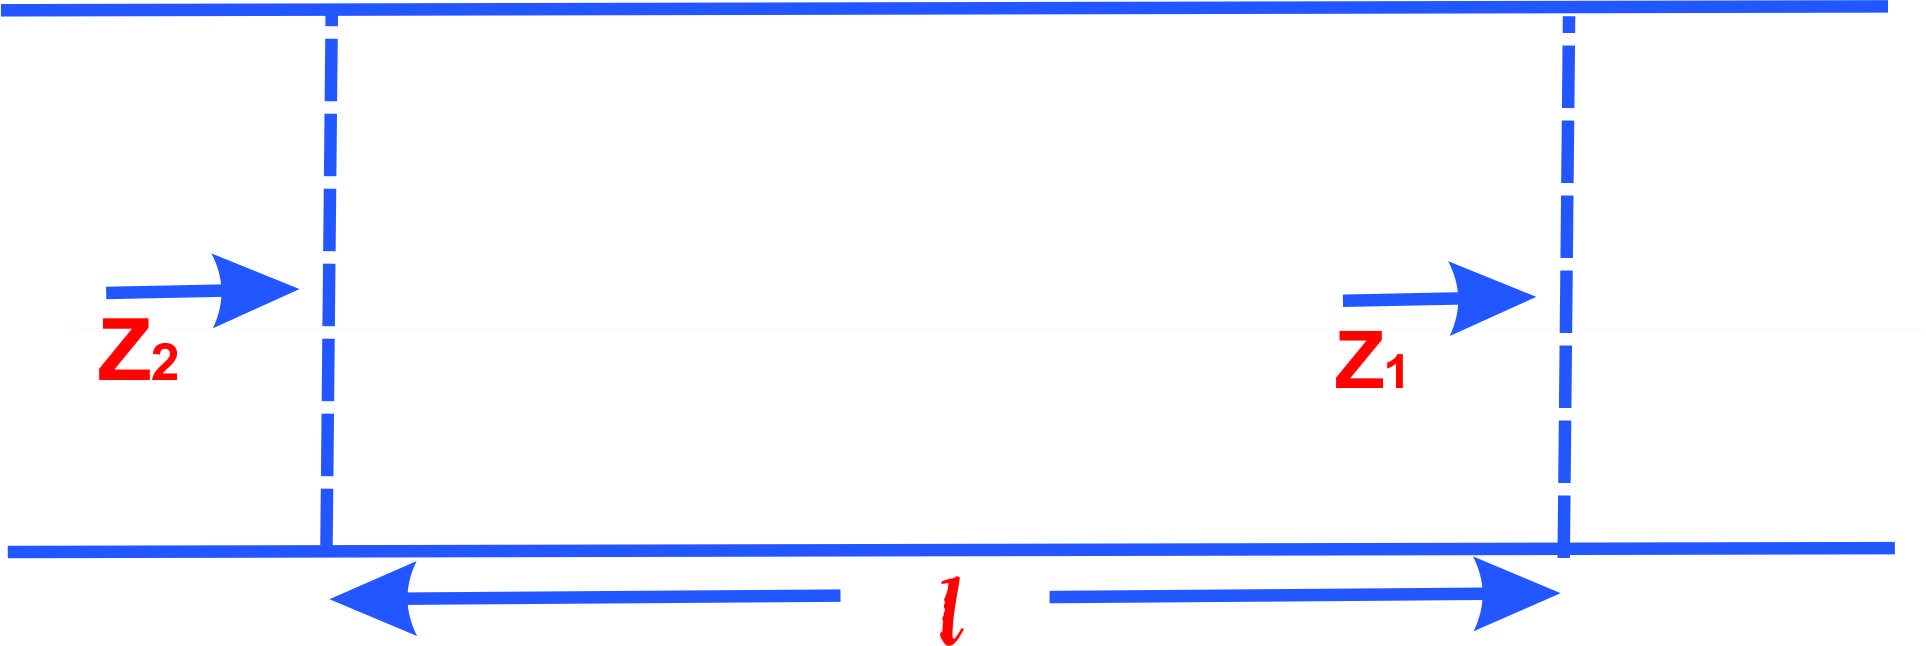
\includegraphics[scale=0.45]{\pathtopartone/graphics/1234}
\caption{General representation of a transmission line}
\label{fig:1234}
\end{figure}
recall from equation~\eqref{eqn:imp} that
\begin{align*}
Z(l) = Z_0\left[\frac{Z_L\cosh(\gamma l) + Z_0\sinh(\gamma l)}{Z_L\sinh(\gamma l) + Z_0\cosh(\gamma l)}\right]
\end{align*}
Let $Z_L = Z_1$ and $Z(l) = Z_2$.
\begin{align}
Z_2 = Z_0\left[\frac{Z_1\cosh(\gamma l) + Z_0\sinh(\gamma l)}{Z_1 \sinh(\gamma l) + Z_0 \cosh(\gamma l)}\right]
\label{eqn:z2norm}
\end{align}
Dividing both sides by $Z_0$
\begin{dmath*}
\frac{Z_2}{Z_0} = \frac{Z_0}{Z_0} \left[\frac{Z_1\cosh(\gamma l) + Z_0\sinh(\gamma l)}{Z_1 \sinh(\gamma l) + Z_0 \cosh(\gamma l)}\right]
= \frac{\frac{Z_1}{Z_0}\cosh(\gamma l) + \frac{Z_0}{Z_0}\sinh(\gamma l)}{\frac{Z_1}{Z_0}\sinh(\gamma l) + \frac{Z_0}{Z_0}\cosh(\gamma l)}
\end{dmath*}
\begin{dmath*}
\bar{Z}_2 = \frac{\frac{Z_1}{Z_0}\cosh(\gamma l) + \sinh(\gamma l)}{\frac{Z_1}{Z_0}\sinh(\gamma l) + \cosh(\gamma l)}
= \frac{\bar{Z}_1\cosh(\gamma l) + \sinh(\gamma l)}{\bar{Z}_1\sinh(\gamma l) + \cosh(\gamma l)}
\end{dmath*}
From equation~\eqref{eqn:z2norm} we can also invert the relationship to get $Z_1$ from $Z_2$ by cross multiplying.
\begin{align*}
Z_2 = Z_0\left[\frac{Z_1\cosh(\gamma l) + Z_0\sinh(\gamma l)}{Z_1 \sinh(\gamma l) + Z_0 \cosh(\gamma l)}\right]
\end{align*}
\begin{dmath*}
Z_2\left[Z_1\sinh(\gamma l) + Z_0\cosh(\gamma l)\right] = Z_0\left[Z_1\cosh(\gamma l) + Z_0\sinh(\gamma l)\right]
\end{dmath*}
\[Z_1Z_2\sinh(\gamma l) + Z_0Z_2\cosh(\gamma l) = Z_0Z_1\cosh(\gamma l) + Z_0^2\sinh(\gamma l)\]

Collect like terms and factorise out $Z_1$ on the left and $Z_0$ on the right-hand side of the equation
\begin{dmath*}
Z_1Z_2\sinh(\gamma l) - Z_1Z_0\cosh(\gamma l) = Z_0^2\sinh(\gamma l) - Z_0Z_2\cosh(\gamma l)
\end{dmath*}
\begin{dmath*}
Z_1\left[Z_2\sinh(\gamma l) - Z_0\cosh(\gamma l)\right] = Z_0\left[Z_0\sinh(\gamma l) - Z_2\cosh(\gamma l)\right]
\end{dmath*}
Make $Z_1$ the subject of the formula
\begin{align}
Z_1 = Z_0\left[\frac{Z_0\sinh(\gamma l) - Z_2\cosh(\gamma l)}{Z_2\sinh(\gamma l) - Z_0\cosh(\gamma l)}\right]
\label{eqn:z1norm}
\end{align}
Multiply the numerator and denominator of equation~\eqref{eqn:z1norm} by $-1$.
\begin{equation}
Z_1 = Z_0\left[\frac{Z_2\cosh(\gamma l) - Z_0\sinh(\gamma l)}{Z_0\cosh(\gamma l) - Z_2\sinh(\gamma l)}\right]\footnotemark
\label{eqn:z1norm2}
\end{equation}
\footnotetext{
Recall, $\cosh-\gamma l = \cosh\gamma l$ and $\sinh-\gamma l = -\sinh-\gamma l$
}
So, equation~\eqref{eqn:z1norm2} can be used to transform impedance between $Z_1$ and $Z_2$ knowing the positive $l$ direction is from load towards the generator.

Now we go to a special case of the transmission lines.

\section{Lossless Transmission Line}
In practice, we want to transfer maximum power from the generator to the load. However, some losses occur in real transmission lines due to ohmic resistances. Every effort is usually made to make sure maximum power is delivered to the load by minimizing these losses. Hence, a good transmission line loss should be very small at its operating frequency.

Once we have this condition in practice, then we can make some simplification to the transmission line problem and come up with an idea of what is called a \emph{lossless transmission line}\index{lossless transmission line} whose ideal loss is zero.

\subsection{Propagation Constant}
The transmission line has four parameters $R, L, G$ and $C$ all in per unit length. $R$ and $G$ are ohmic values in the primary constants which is the resistance between the two ends of the conductors and the leakage current in the dielectric separating the two conductors respectively. Hence, power-losing elements exist because of the resistance and conductance. The inductance and capacitance exchange energy between themselves but do not result in any loss. Ideally, a line will be lossless if $R = G = 0$.

Substituting $R$ and $G$ as zero in the propagation constant\index{propagation constant} from equation~\eqref{eqn:gamma} given as follows simplifies to,
\begin{dmath*}
\gamma = \sqrt{(R + \jmath\omega L)(G + \jmath\omega C)}
= \sqrt{(\jmath\omega L)(\jmath\omega C)}
= \jmath\omega\sqrt{LC}
\end{dmath*}
Recall that the propagation constant is a complex quantity represented as,
\begin{align*}
\gamma = \alpha + \jmath\beta
\end{align*} 
Therefore,
\begin{align*}
\alpha + j\beta = \jmath\omega\sqrt{LC}
\end{align*}
so,
\begin{align*}
\alpha = 0\quad\text{and}\quad\beta = \omega\sqrt{LC}
\end{align*}

With no loss, there is no reason for the wave amplitude to reduce on the transmission line since the attenuation constant, $\alpha = 0$. Hence, there is a sustained propagation of electromagnetic waves along the transmission line. We can further simplify the phase constant as follows
\begin{align*}
\beta &= \omega\sqrt{LC}\quad\text{But }\beta\text{ = }\frac{2\pi}{\lambda}\text{ and }\omega\text{ = }2\pi f\\
\frac{2\pi}{\lambda} &= 2\pi f\sqrt{LC}\\
\frac{1}{\lambda} &= f\sqrt{LC}\footnotemark
\end{align*}
\footnotetext{
$2\pi$ will cancel out on both sides
}
Recall, $\lambda f = v$ which is the velocity of the wave in the transmission line. Thus
\begin{align*}
\lambda f = \frac{1}{\sqrt{LC}} = v
\end{align*}
The velocity of the wave in the transmission line is related to the inductance and capacitance of the transmission line. Hence the velocity is fixed once the inductance and capacitance are given.

\emph{Can we vary load $L$ and $C$ to vary $v$?} Not really, $L$ and $C$ are coupled. Varying $C$ changes $L$ and varying $L$ changes $C$ to make $v$ a constant of the transmission line. The velocity is decided by the field condition in the transmission line and is fixed by the boundary condition. For instance, with varying separation between the two conductors, the mutual inductance will vary and at the same time, the separation between the two conductors vary thereby varying the capacitance. Hence, $L$ and $C$ of the transmission line are not independent quantities.

\subsection{Characterisitic Impedance}\index{characteristic impedance}
We then calculate the characteristic impedance on a lossless transmission line which is given as,
\begin{dmath*}
Z_0 = \sqrt{\frac{R + \jmath\omega L}{G + \jmath\omega C}}
= \sqrt{\frac{\jmath\omega L}{\jmath\omega C}}\quad\text{Since }R\text{ = }0\text{ and }G\text{ = }0
= \sqrt{\frac{L}{C}} \quad\textnormal{(real quantity)}
\end{dmath*}
Therefore, for a lossless line, it can be observed that $Z_0$ is real. We do not have any ohmic resistance or conductance in the line and yet it is at this point we have a characteristic impedance that is real (that is, pure ohmic loss). Hence, the wave which travels forward or backwards always sees a characteristic impedance that is a real impedance like resistance. This makes sense since we have a line carrying only forward waves which will go forever and no energy is reflected. That is, power somewhere is going to get dumped at the load end. So if we have a real quantity for $Z_0$, it means that power is completely transferred to the line. It does not mean that power is lost in the line. So for a lossless line, if the impedance on the line is measured, something more like resistance will be measured.

Now, we go to a case where little loss is accepted in the transmission line and then find the derivations for $\gamma$ and $Z_0$.

\section{Low-loss Transmission Line}\index{low-loss transmission line}
$R\ll\omega L$, $G\ll\omega C$ are the two conditions for a low-loss transmission line. So we derive the propagation constant of this line.

\subsection{Propagation Constant}\index{propagation constant}
Using equation~\eqref{eqn:gamma}, we have:
\begin{dmath}
\gamma = \sqrt{(R + \jmath\omega L)(G + \jmath\omega C)}
= \sqrt{{(\jmath\omega L)(\jmath\omega C)\left(1 + \frac{R}{\jmath\omega L}\right)\left(1 + \frac{G}{\jmath\omega C}\right)}}
= \sqrt{{(\jmath\omega L)(\jmath\omega C)\left(1 - j\frac{R}{\omega L}\right)\left(1 - j\frac{G}{\omega C}\right)}}\footnotemark
\label{eqn:lowlossgamma}
\end{dmath}
\footnotetext{
Recall $\frac{1}{\jmath} = -\jmath$
}
The expressions $\left(1 - j\frac{R}{\omega L}\right)^{\frac{1}{2}}$ and $\left(1 - j\frac{G}{\omega C}\right)^{\frac{1}{2}}$ in equation~\eqref{eqn:lowlossgamma} can be expressed as a power series. Recall from Binomial expansion the a power series with fraction power can be expressed as follows where $x$ is the fractional part.
\begin{dmath*}
(1 + x)^{\frac{1}{2}} = \Comb{\frac{1}{2}}{0}(1)^{\frac{1}{2}}x^0 + \Comb{\frac{1}{2}}{1}(1)^{{\frac{1}{2}} - 1}x^1 + \ldots
\end{dmath*}
Where $\Comb{\frac{1}{2}}{0}(1)^{\frac{1}{2}}x^0 = 1$ and $\Comb{\frac{1}{2}}{1}(1)^{\frac{1}{2} - 1}x = \Comb{\frac{1}{2}}{1}(1)x$.

Let's expand the combination $\Comb{\frac{1}{2}}{1} x$
\begin{dmath*}
\Comb{\frac{1}{2}}{1} x = \begin{pmatrix}\frac{1}{2}\\1 \end{pmatrix}x = \frac{\frac{1}{2}! x}{(\frac{1}{2} - 1)!1!} = \frac{\frac{1}{2}(\frac{1}{2} - 1)! x}{(\frac{1}{2} - 1)!1!} = \frac{1}{2}x
\end{dmath*}

Thus,
\[(1 + x)^{\frac{1}{2}} = 1 + \frac{1}{2}x + \ldots\]
and
\[(1 - x)^{\frac{1}{2}} = 1 - \frac{1}{2}x + \ldots\]

Hence from the equation~\eqref{eqn:lowlossgamma}
\[jw\sqrt{LC}\left(1 - \jmath\frac{R}{wL}\right)^{\frac{1}{2}}\left(1 - \jmath\frac{G}{wC}\right)^{\frac{1}{2}}\]
Let $x = \jmath\frac{R}{\omega L}$ and $x' = \jmath\frac{G}{\omega C}$
\begin{dmath*}
\left(1 - \frac{\jmath R}{\omega L}\right)^{\frac{1}{2}} = 1 - \frac{1}{2}\frac{\jmath G}{\omega C} + \ldots
\end{dmath*}
and
\begin{dmath*}
\left(1 - \frac{jG}{\omega C}\right)^{\frac{1}{2}} = 1 - \frac{1}{2}\frac{\jmath R}{\omega L} + \ldots 
\end{dmath*}
Thus, equation~\eqref{eqn:lowlossgamma} becomes
\begin{dmath*}
\gamma = jw\sqrt{LC}\left(1 - \jmath \frac{R}{2\omega L} + \ldots\right)\left(1 - j\frac{G}{2\omega C} + \ldots\right) = jw\sqrt{LC} \left[1- \left(\frac{\jmath R}{2\omega L}\right) - \left(\frac{\jmath G}{2\omega C}\right) + \left(\frac{\jmath R}{2\omega L}\right)\left(\frac{\jmath G}{2\omega C}\right)\right]
\end{dmath*}
Recall that two combination terms were used earlier because of the complex variable $\frac{jR}{wL}$ and $\frac{\jmath G}{\omega C}$, the product of $\frac{\jmath R}{2\omega C}$ and $\frac{\jmath G}{2\omega L}$ tends to zero since $R \ll wL$ and $G \ll \omega C$ for a low loss transmission line.

Thus,
\begin{dmath}  
\gamma = \jmath\omega\sqrt{LC} \left[1- \frac{\jmath R}{2\omega L} - \frac{\jmath G}{2\omega C}\right] = \jmath\omega\sqrt{LC} - \jmath\frac{R}{2\omega L}\left(\jmath\omega\sqrt{LC}\right) - j\frac{G}{2\omega C}\left(\jmath\omega\sqrt{LC}\right)
\end{dmath}
Expressing $L = \sqrt{L} \times \sqrt{L}$ and $C = \sqrt{C} \times \sqrt{C}$, we have
\begin{dmath*}
\gamma = \jmath\omega\sqrt{LC} + \frac{R\sqrt{L}\sqrt{C}}{2\sqrt{L}\sqrt{L}} + \frac{G\sqrt{L}\sqrt{C}}{2\sqrt{C}\sqrt{C}}
= \jmath\omega\sqrt{LC} + \frac{1}{2}R\sqrt{\frac{C}{L}} + \frac{G}{2}\sqrt{\frac{L}{C}} 
\end{dmath*}

Recall that $\gamma = \alpha + j\beta$, therefore,
\begin{align*}
\jmath\omega\sqrt{LC} + \frac{1}{2}R\sqrt{\frac{C}{L}} + \frac{G}{2}\sqrt{\frac{L}{C}} = \alpha + \jmath\beta
\end{align*}
So,
\begin{align}
\alpha &= \frac{1}{2}R\sqrt{\frac{C}{L}} + \frac{1}{2}G\sqrt{\frac{L}{C}}\label{eqn:lowlossalpha}\\
\beta &= \omega\sqrt{LC}
\end{align}
Compared to the lossless transmission line where $\alpha = 0$, there is a value for the attenuation constant. Also, we have that $\beta = \omega\sqrt{LC}$ for both cases of lossless and low-loss, which means that the phase constant does not change when we introduce low-loss to the transmission line. Hence, if we are interested in only the phase constant for a low-loss line, it can be treated as a lossless transmission line. However, for a low-loss transmission line $\alpha \neq 0$, there is that small loss so that as one travels with the wave, amplitude reduces slowly at $e^{-\alpha}$.

\subsection{Characterisitic Impedance}\index{characteristic impedance}
Recall, $Z_0 = \sqrt{\frac{L}{C}}$ for a lossless line, substituting it in equation~\eqref{eqn:lowlossalpha}, we have,
\[\alpha = \frac{1}{2}R\sqrt{\frac{C}{L}} + \frac{1}{2}G\sqrt{\frac{L}{C}} = \frac{1}{2}\left(\frac{R}{Z_0} + GZ_0\right)\]
Therefore,
\[\gamma = \jmath\omega\sqrt{LC} + \frac{1}{2}\left(\frac{R}{Z_0} + GZ_0\right)\]
So if $R$ and $G$ are known and $Z_0$ for the lossless line has been determined, we can use $\alpha = \frac{1}{2}(\frac{R}{Z_0} + GZ_0)$ to calculate $\alpha$ for the low-loss line.
\begin{align*}
Z_0 = \sqrt{\frac{R + \jmath\omega L}{G + \jmath\omega C}} = \sqrt{\frac{\jmath\omega L(1 - \jmath\frac{R}{\omega L})}{\jmath\omega C(1 - \jmath\frac{G}{\omega C})}}
\end{align*}
$j\omega$ will cancel out, leaving us with
\begin{dmath*}
Z_0 = \sqrt{\frac{L}{C}}\sqrt{\frac{1 - j\frac{R}{\omega L}}{1 - j\frac{G}{\omega C}}} =\sqrt{\frac{L}{C}}\left(1 - \jmath\frac{R}{\omega L}\right)^{\frac{1}{2}}\left(1 - \jmath\frac{G}{\omega C}\right)^{-\frac{1}{2}} 
\end{dmath*}
From Binomial expansion, we have that:
\begin{align*}
Z_0 = \sqrt{\frac{L}{C}}\left(1 - \jmath\frac{R}{2\omega L} + \ldots\right)\left(1 - \jmath\frac{G}{2\omega C} + \ldots\right)
\end{align*}
\begin{align*}
= \sqrt{\frac{L}{C}}\left(1 - \jmath\frac{R}{2\omega L} - \jmath\frac{G}{2\omega C} + \text{\ldots (\it{smaller terms})}\right)
\end{align*}
The characteristic impedance is no more real but complex. Its real value is the same as that of a lossless line. We have a small imaginary part which implies the presence of losses in the transmission line.

From now on, when given a transmission line problem, we assume it to be lossless unless we are told specifically that the line is lossy.

\section*{Exercises}
\begin{ExerciseList}
\Exercise[label={ex41}]
Show that for a lossless transmission line, the velocity of the wave is a function of L and C i.e. $\left(v = \frac{1}{\sqrt{LC}}\right)$.

\Exercise[label={ex42}]
Given a transmission line with primary constants, $R = 0.00259\varOmega/$m, $L = 2\mu H/$m, $G = 0$ and $C = 5.56pF/$m operating at a frequency of 5kHz, find the characteristic impedance, propagation constant (attenuation and phase constant), velocity of propagation, and wavelength.
\Answer[ref={ex42}]
(a) $Z_0 = 600\angle-1.2^o\varOmega$ (b) $\gamma = 1.048\times10^{-4}\angle88.8^o/$m (c) $v = 2.998\times10^8$m/s and (d) $\lambda = 59.98$km.

\Exercise[label={ex43}]
Prove that for both a lossless and a low-loss transmission line, the phase constant remains the same while the attenuation constant changes.
\end{ExerciseList}
